\documentclass[conference]{IEEEtran}

\usepackage{grffile}
\usepackage{epstopdf}
\usepackage{graphicx}
\usepackage{amsmath} % split in equation environment
\usepackage{amssymb}
\usepackage{mathrsfs}
%\usepackage{hyperref}
\usepackage{multirow}
\usepackage{lipsum}
\usepackage{cleveref}
\usepackage{ wasysym }
\usepackage[numbers]{natbib}% citet
\usepackage{comment}
\usepackage{float}
%\usepackage[colorlinks]{hyperref}
\usepackage[colorinlistoftodos]{todonotes}%http://www.texample.net/tikz/examples/todo-notes/

\usepackage{tikz}
\usepackage{pgfplots}
\usepgfplotslibrary{patchplots}

\usepackage{multirow}

\DeclareMathAlphabet{\mathpzc}{OT1}{pzc}{m}{it}
\newcommand{\soc}{\mathpzc{soc}}
\newcommand{\rload}{\mathpzc{rLoad}}
\newcommand{\fl}{\mathpzc{flow}}
\newcommand{\lpc}{LP-PEMS}
\usepackage{color,soul} % for highlighting using \hl
\usepackage{balance}


\usepackage{array}
\usepackage{mdwmath}
\usepackage{mdwtab}
\usepackage[caption=false,font=footnotesize]{subfig}

% correct bad hyphenation here
% \hyphenation{op-tical net-works semi-conduc-tor}
\addtolength{\topmargin}{0.025in}

% Uncomment bellow for 1.5=line spacing (draft)
%\linespread{1.3}

\begin{document}

% paper title
% Titles are generally capitalized except for words such as a, an, and, as,
% at, but, by, for, in, nor, of, on, or, the, to and up, which are usually
% not capitalized unless they are the first or last word of the title.
% Linebreaks \\ can be used within to get better formatting as desired.
% Do not put math or special symbols in the title.
%\title{A Dynamic Controller Model to Optimize the Neighborhood Self-Consumption of Power}
%\title{Extraction of Optimal Energy Management Rules using Fuzzy Control and Differential Evolution}
\title{Enhancing Power Flow Simulations\\Using Function Mapping}


\author{
\textsc{Michael Bardwell}\\ % Your name
%\normalsize \href{mailto:bardwell@ualberta.ca }{bardwell@ualberta.ca }\\
\textsc University of Alberta - Department of Electrical and Computer Engineering \\
}
% author names and affiliations
% use a multiple column layout for up to three different
% affiliations
\author{\IEEEauthorblockN{Michael Bardwell\IEEEauthorrefmark{1}, 
Petr Musilek\IEEEauthorrefmark{1}\IEEEauthorrefmark{2}}
\IEEEauthorblockA{\IEEEauthorrefmark{1}Department of Electrical and Computer Engineering, University of Alberta, Edmonton, AB, Canada}{\IEEEauthorrefmark{2}Department of Cybernetics, Faculty of Science, University of Hradec Kr\'{a}lov\'{e}, Czech Republic}
}

% conference papers do not typically use \thanks and this command
% is locked out in conference mode. If really needed, such as for
% the acknowledgment of grants, issue a \IEEEoverridecommandlockouts
% after \documentclass

% for over three affiliations, or if they all won't fit within the width
% of the page, use this alternative format:
% 
%\author{\IEEEauthorblockN{Michael Shell\IEEEauthorrefmark{1},
%Homer Simpson\IEEEauthorrefmark{2},
%James Kirk\IEEEauthorrefmark{3}, 
%Montgomery Scott\IEEEauthorrefmark{3} and
%Eldon Tyrell\IEEEauthorrefmark{4}}
%\IEEEauthorblockA{\IEEEauthorrefmark{1}School of Electrical and Computer Engineering\\
%Georgia Institute of Technology,
%Atlanta, Georgia 30332--0250\\ Email: see http://www.michaelshell.org/contact.html}
%\IEEEauthorblockA{\IEEEauthorrefmark{2}Twentieth Century Fox, Springfield, USA\\
%Email: homer@thesimpsons.com}
%\IEEEauthorblockA{\IEEEauthorrefmark{3}Starfleet Academy, San Francisco, California 96678-2391\\
%Telephone: (800) 555--1212, Fax: (888) 555--1212}
%\IEEEauthorblockA{\IEEEauthorrefmark{4}Tyrell Inc., 123 Replicant Street, Los Angeles, California 90210--4321}}

% use for special paper notices
%\IEEEspecialpapernotice{(Invited Paper)}

% make the title area
\maketitle
%\todo[inline]{Capture the model purpose and think in a better title}%

%\listoftodos

% As a general rule, do not put math, special symbols or citations
% in the abstract
\begin{abstract}
The main contribution of this paper is demonstrating the approximation of the power system load flow (PSLF) function. The topological correspondence of radial, electrical power grids is captured with an Artificial Neural Network. A hyperparameter grid search was used to confirm the optimal training conditions. It was discovered that even for large radial networks, the identity linear regression outperforms non-linear regression under reasonable training circumstances. This indicates PSLF is a relatively linear function even when the feature space is large. The findings were used to develop a Python-based framework to autonomously handle simulation function mapping, which allows for model re-use making the simulation process less computationally expensive and less time-consuming on average.
%Popular MPPT algorithms like Perturb and Observe are trialed on the Beaglebone Green (BBG) and ESP8266 Feather Huzzah (ESP) and each segment necessary for the system to operate is timed. It is shown that API calls are the major efficiency cap, covering over 90\% of the runtime making it hard to cut the perturbation period down

%MPPT code is developed for two IoT devices, and is segmented by operation during discussion to demonstrate the time between online, offline and hybrid algorithms A buck converter battery charge circuit was designed with a calculated minimum perturbation period of $18.5 us$, along with a minimum duty cycle perturbation step of $0.026$. An independent study on high resolution irradiance data was used to determine the average irradiance slope. Python code is developed for the Beaglebone Green and C code is created for the ESP8266 Feather Huzzah. Capabilities of alternative IoT hardware are discussed. Statistical analysis is performed on historical irradiance data to deliver irradiance slope estimates within a confidence interval. A community test case shows that efficient MPPT using inexpensive IoT hardware is possible, with the added benefit of readily available data for digital services.
\end{abstract}
% no keywords

% For peer review papers, you can put extra information on the cover
% page as needed:
% \ifCLASSOPTIONpeerreview
% \begin{center} \bfseries EDICS Category: 3-BBND \end{center}
% \fi
%
% For peerreview papers, this IEEEtran command inserts a page break and
% creates the second title. It will be ignored for other modes.
\IEEEpeerreviewmaketitle


\section{Introduction}
\label{sec:intro}
Modern simulation techniques are expensive. High resolution, complex simulations can take on the order of hours or days to come to completion and require advanced, costly computers. When these simulations are completed, it is likely the researcher or practitioner will run another, restarting the whole process. The institutional solution is to purchase faster, more expensive computers. While the outputs of the simulation are the desired results, no conclusive research has been done on capturing the simulation model for re-use. It is viewed as a black box, often deleted post-simulation only for the same model to be rerun later on a different input sequence.

Today's simulation models are handled in engines like MATLAB Simulink. The engine handles highly multivariate, nonlinear equations, masked by a graphical user interface and solved using numerical methods. Advanced regression techniques and computing power has made it possible to capture extremely high-dimensional, nonlinear equations. This paper explores the regression techniques successful in function approximation of the topological correspondence in electric power grids.

\begin{equation} f(x) = \sum_{i =0}^{z}w_{i}^{T} \cdot \phi_{i}(x) \label{form:regr} \end{equation} 

The general regression formula is shown in Eq. (\ref{form:regr}). The function is linear with respect to the weights $w$, and the basis functions $\phi(x)$. One example of an estimator consistent with this formula are one-layer Artificial Neural Networks (ANN) and will be discussed later in this paper.

The electric power grid is governed by the power system load flow (PSLF) equation in Eq. (\ref{form:nlpfeqn}). PSLF defines the relationship between the input power vector $S_{i}$, and the output voltage vector $V_{i/k}$. The user creates a Y-bus admittance matrix $Y_{ii/ik}$, by selecting the bus connection topology like the radial topology in Fig. \ref{fig:radnetwork}, where each circle represents a node in the power system network. Our focus is to capture the unique correspondence between houses, embedded in $Y$, using function mapping.

\begin{equation} V_i = \frac{1}{Y_{ii}} \cdot \left(\frac{S_i^*}{V_i^*} - \displaystyle\sum_{k=1,k \neq i}^{n} Y_{ik} \cdot V_k\right) \label{form:nlpfeqn} \end{equation}

\begin{figure}[h]
	\centering
	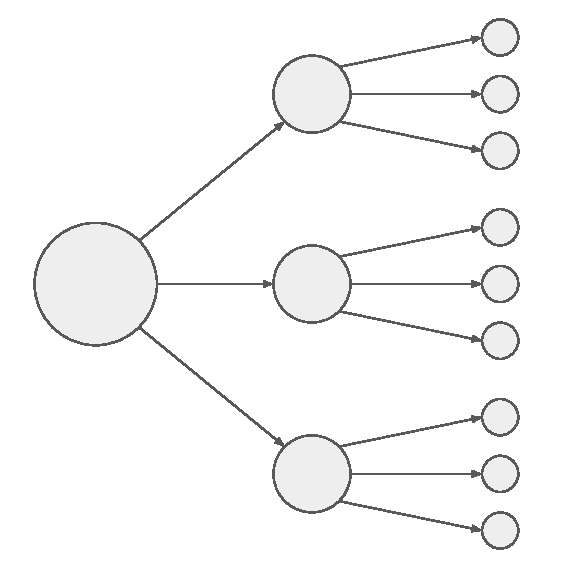
\includegraphics[width=5cm]{radialnetwork.pdf}
	\caption{A sample radial network}
	\label{fig:radnetwork}
\end{figure}

There are many function approximation techniques, starting in statistics with methods like Nonlinear Least Squares and Maximum Likelihood Estimates which belong to a broader class called M-estimators \cite{haya2000}. Radial basis functions are used in \cite{mann1999} to model nonlinear voiced speech sounds. In \cite{chen1994}, Chen develops a backpropagation technique for multi-layer perceptron function approximation. Concepts of extrema equivalence are developed to estimate the complexity of a function in \cite{zhang2004}, thereby providing an empirical method to select ANN network size and toplogy. A statistical perspective on many of the aforementioned techniques is provided by Cheng in \cite{cheng1994}; for example, assume there is a constant $V$, such that $f(x)/V$ is inside the convex hull of a trained one-layer ANN represented as $f_{M}$, amongst a few other assumptions. We can say the approximation error is bounded as:

\begin{equation} \|f - f_{M}\| \leqslant \frac{V}{\sqrt{M}}, \label{form:1layerannbound} \end{equation}

\noindent where M is the number of neurons in the hidden layer.

Artificial neural networks are a good choice for function approximation due to their adjustable basis function nature \cite{barr1994}. This is excellent for our application as there is uncertainty in the nature of the PSLF-based function to be approximated. Before training, hyperparameter adjustments prepare the underlying basis structure and training tunes the basis functions.

Once a function has been approximated, it is important to make it as usable as possible. A Python program was developed to autonomously handle the PSLF function approximation process. The program is summarized in Fig. \ref{fig:infoflow}.

\setcounter{figure}{2} % because this figure will float to a later page, it needs to be artificially numbered later
\begin{figure*}[h]
	\centering
	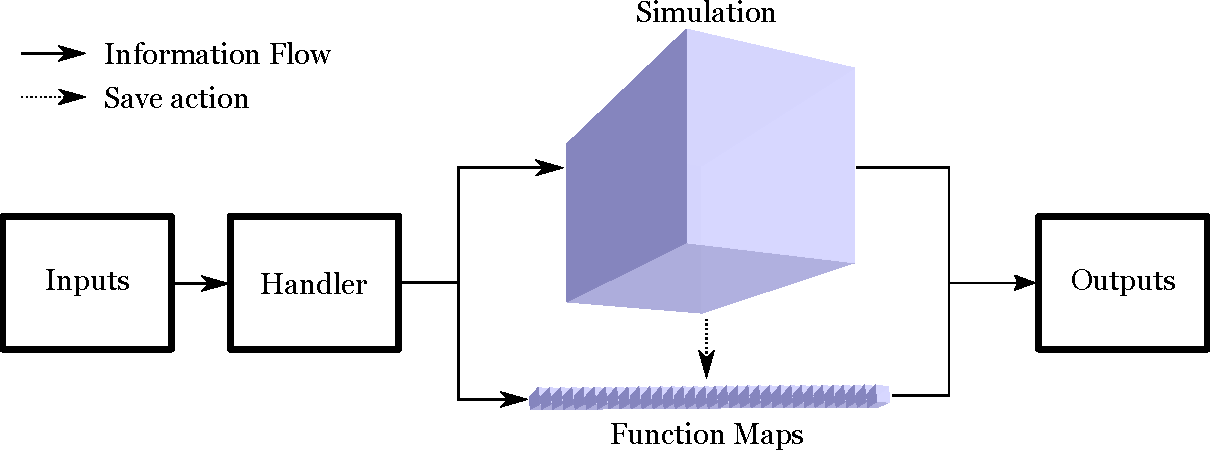
\includegraphics[width=11cm]{informationflow.pdf}
	\caption{Flow of information in Simulation Handler Python program. The user provides a simulation model and input samples and the handler automates the PSLF process. The output is a set of node voltages concurrent with the samples seen at the input	}
	\label{fig:infoflow}
\end{figure*}

In Section \ref{sec:relwork} the nuances of function approximating are discussed. In Section \ref{sec:model} the experimental method is outlined and the results are tabulated in Section \ref{sec:results}. Section \ref{sec:conc} summarizes the contributions of this paper. The research is wrapped in an open-source Python package available through \textit{pip install simhandler} or GitHub\footnote{https://github.com/mbardwell/intelligent-simulation-handler}.

\section{Background}
\label{sec:relwork}
\vspace{-2em} % compensate for extra space at background (don't know why it's there...)
A mapping is a rule of correspondence between input and output vectors. To function map a simulation model, two sets of vectors $a_{i} \in R^{p}$, $b_{i} \in R^{q}$ are required: a finite input data set $\left\{a_{0}, a_{1}, \ldots, a_{m}\right\}$ and a finite output data set $\left\{b_{0}, b_{1}, \ldots, b_{n}\right\}$; the output set is calculated by passing the input set through a well-defined simulation model. $m$, $n$ are the number of input/output features in the simulation model respectively and the length of each vector in either set is defined as the number of samples and is orthogonal to $m$, $n$. For example, a Modified National Institute of Standards and Technology (MNIST) identifier might have a 1000 pixels per image and 10 possible outcomes (digits 0-9), given them $m$ = 1000 and $n$ = 10 respectively. The length of vector $a_0 = 100$, for example, which could be the top left pixel from 100 pictures; $b_0$ would be 100 respective classifications.

The more non-linear the simulation model, the more samples required for function mapping to meet high accuracy goals. For example, imagine the simulation model is a simple, two-dimensional linear function. From Eq. (\ref{form:regr}), assuming $\phi(x) = \{1, x\}$

\begin{equation} f(x) = w_{0} + w_{1} x. \label{form: line} \end{equation}

To determine the bias $w_{0}$ and weight $w_{1}$, you only require two, linearly independent, m-dimensional data points and you have a perfect function mapping of the model. Now let us imagine a more likely scenario for a simulation model,  something like the noisy function in Fig. \ref{fig:simdata}.

\setcounter{figure}{1} % Because this figure comes after the 'information flow' figure in text but not after compile
\begin{figure}[H]
	\centering
	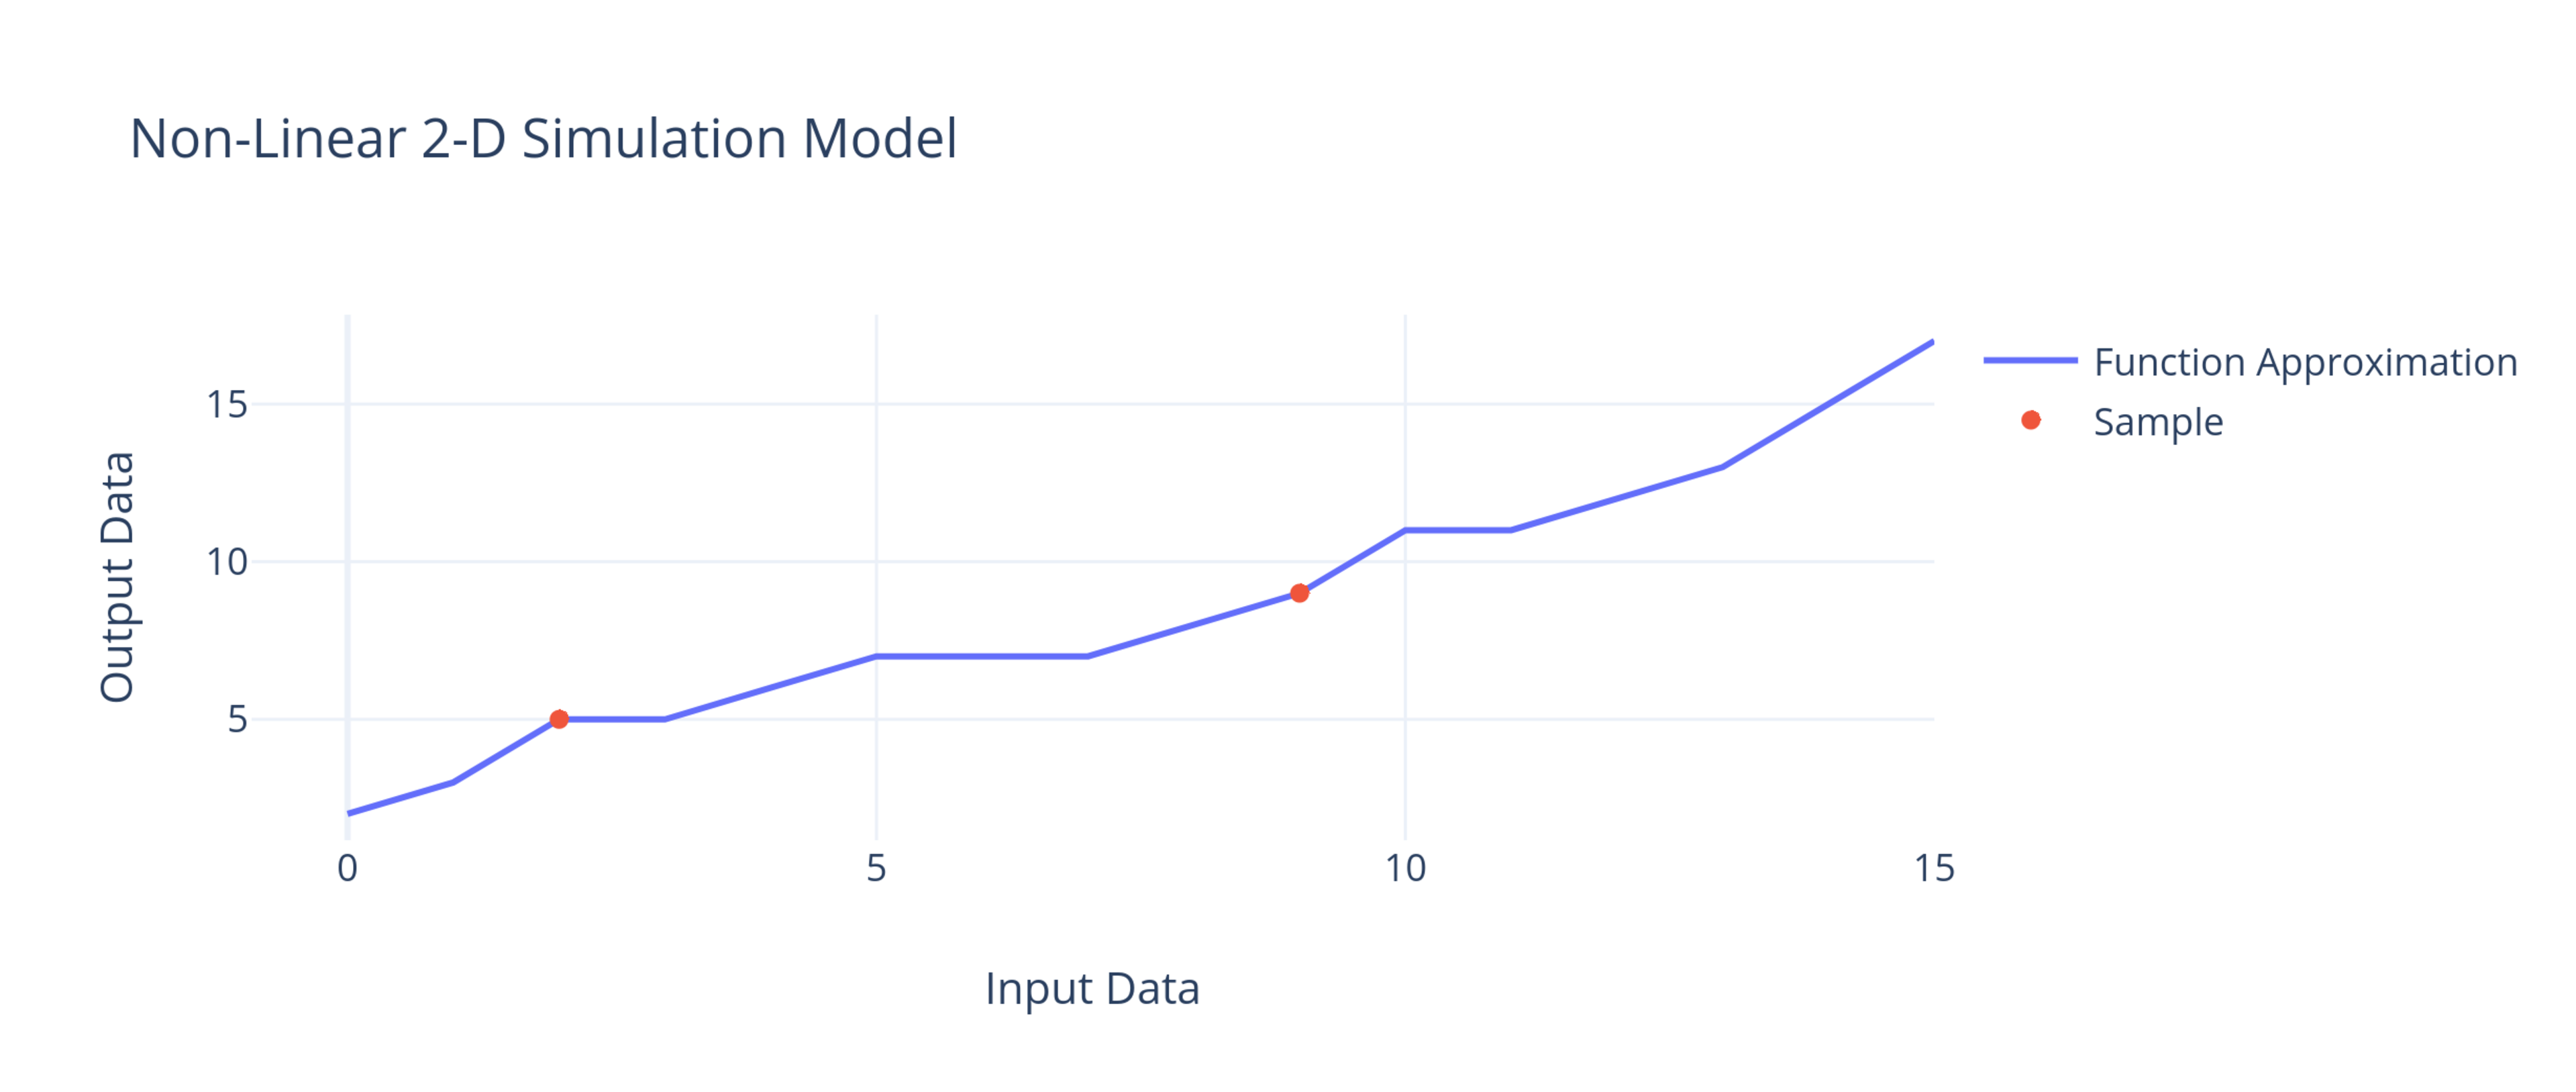
\includegraphics[width=9cm]{simdata.pdf}
	\caption{Sample simulation data}
	\label{fig:simdata}
\end{figure}

It is obvious by inspection that any line, like one drawn between the two sample dots in Fig. \ref{fig:simdata}, would be an underfitted approximation of the correspondence in this simulation. To get a better fit that encompasses the valley at $x = 7$ or the peak at $x  =10$, for example, more samples from the simulation model are required. This type of underfitting is exponentially amplified in higher dimensions, due to the curse of dimensionality, so with larger features spaces, even more data is required.

To map the PSLF equation, a feed-forward ANN is fed with electric power system data. Pre-processing for this data is minimal as each feature is already geometrically balanced; also using per unit ensures the input/output values are close to 1. The network is trained using simple backpropagation. A Monte Carlo approach is taken to fill $S_{i}$ using a uniform distribution with support $x \in [0, 1)$; the stochastic approach optimizes the efficiency of mapping nonlinear functions, much like random search optimizes efficiency for hyperparameter exploration \cite{berg2012}.

There are many variations in power system topology, see Table \ref{table:sim model}. The objective in this paper is to provide the experimental procedure for function mapping a radial feeder network with resistive-only lines. The methodology should naturally extend to other variations as well. For this paper, an accuracy of $10^{-2}$ was arbitrarily selected as sufficient. For example, if the base voltage for a distribution line is 35 kV, the upper bound on the estimation error would be 350 V. This factor can be used to tell the network when to stop training.

\begin{table}[h]
\centering
\caption[Power system network parameters]{Power system network parameters}
 \begin{tabular}{|c c|} 
  \hline
PS Parameter & Examples \\ %[0.5ex] 
 \hline\hline
Bus Topology & Main-Tie-Main, Ring, Primary Loop \\
 \hline
Feeder Network & Radial, Parallel, Ring, Meshed  \\ 
 \hline
Line Characteristics & Resistance, Reactance, Length, Maximum Power  \\
\hline
Line Support & Shunt/Series Compensation \\
\hline
Storage Parameters & BESS's, Flywheels, Compressed Air \\
\hline
Generator Availability & Minimum/Maximum Real and Reactive Power \\
\hline
\end{tabular} \vspace{1mm}
\label{table:sim model}
\end{table}

Mean-square error (MSE), also known as the $\ell_{2}$ or Euclidean norm is the accuracy metric used for regression evaluation. It is optimal for function approximation as it is more sensitive to outliers than mean absolute error. Root-MSE (RMSE) will be used for analysis, considering the fact that it is in the same units as the feature space.

To demonstrate the accuracy capabilities of nonlinear function mapping, the results are compared to an identity linear regression (ILR) with m-dimensions, which is derived by setting $\phi_{i}(x) = x_{i}$ in Eq. (\ref{form:regr})

\begin{equation} f(x) = w_{0} + \sum_{i =1}^{m}w_{i}^{T} \cdot x_{i}. \label{form: idnregr} \end{equation}

For smaller-featured systems, ILR may out-perform the ANN. This is because PSLF with very small systems tends to have little noise; also ILR is fitted to the data, which unlike gradient descent used in ANN training is an exact process. ILR is fitted using the normal equation.

\begin{equation} \hat{\theta} = (\textbf{X}^T \cdot \textbf{X})^{-1} \cdot{X}^T \cdot \textbf{y} \label{form:normaleqn} \end{equation}

One non-obvious trade off between ILR and ANN is the expensive nature of normal equation calculations; for ILR a matrix inversion is required, which in Big-O notation is between $O(m^{2.4})-O(m^{3})$. The processing cost of ANN training scales linearly, or $O(m)$. This is demonstrated by the timing comparison in Fig. \ref{fig:featvstime}.

\setcounter{figure}{3} % Last figure that must be adjusted because of floating 'information flow' figure
\begin{figure}[H]
	\centering
	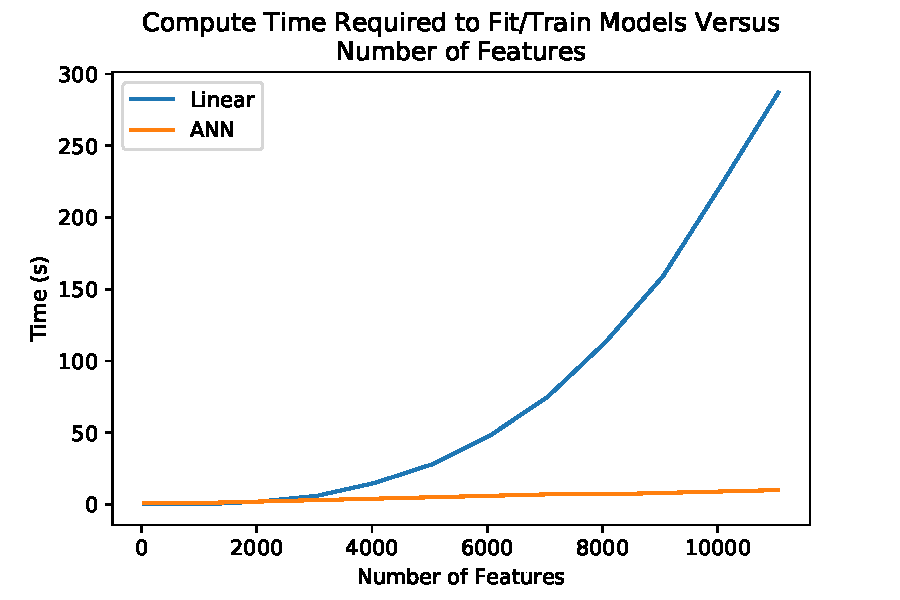
\includegraphics[width=9cm]{featuresversustime.pdf}
	\caption{Compute time required to fit an ILR (\textit{Linear} in legend) using the normal equation versus train an ANN using backpropagation}
	\label{fig:featvstime}
\end{figure}

\section{Experimental Method}
\label{sec:model}
The generic approach to function approximating PSLF equations is outlined in Fig. \ref{fig:expapproach}. To achieve results in swift fashion, a hyperparameter search will be automated using an open-source Python library, Talos.

\begin{figure}[H]
	\centering
	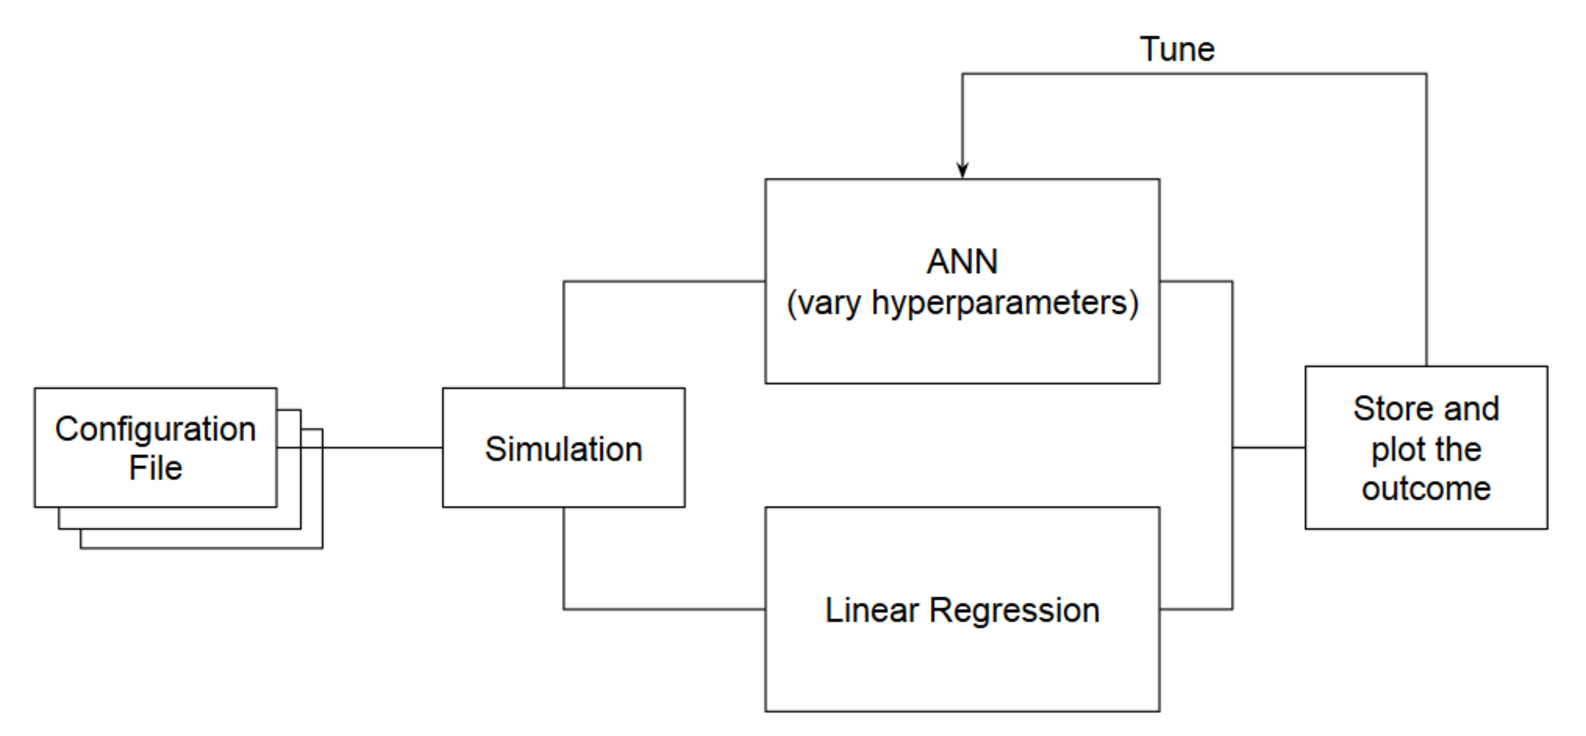
\includegraphics[width=9cm]{experimentalprocedure.pdf}
	\caption{General approach to function mapping PSLF equations}
	\label{fig:expapproach}
\end{figure}

According to \cite{chen1994}, \cite{du2014}, three-layer ANN's are considered universal approximators. Naturally, this would be a good starting number of hidden layers, however preliminary tuning with ILR, which is similar to a one-layer ANN has shown reasonable results. So the number of hidden layers will be tuned between 1-3. 

Sample size is also important. Since a Monte Carlo approach is taken to fill $S_{i}$, the theoretically optimum $S_{i}$ would be an infinite set of samples, which would then be used to fit/train the approximation. However, since this is practically unrealistic, a preliminary study was done to determine the time it takes to calculate the output set $V_{i/k}$ of various sizes. The relationship between processing time and set size can then be used to select a reasonable sample size. Note that the intention of this study is to observe the high extrema of accuracy, so a high sample/small feature space approach was taken.

\begin{figure}[h]
	\centering
	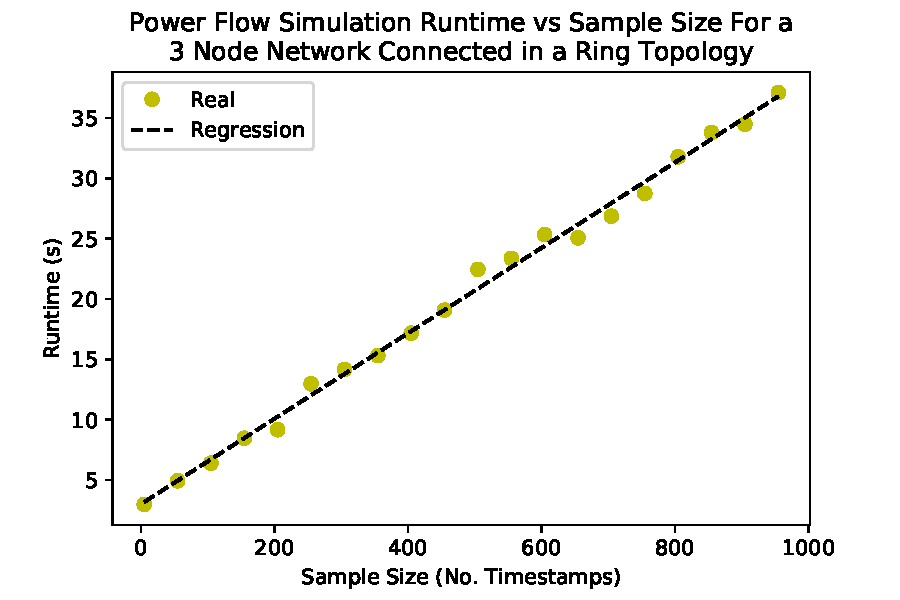
\includegraphics[width=9cm]{pslfruntimevssamples.pdf}
	\caption{Power system load flow analysis time requirements as a function of sample size. Run on Intel Core i5 and 16 GB of RAM}
	\label{fig:pslfruntime}
\end{figure}

The results from Fig. \ref{fig:pslfruntime} show the runtime increases around $0.034~s$ per sample for a very small network. Another study showed an increase of $0.016~s$ per feature. This gives us the following runtime equation: $t(s) = 0.034\cdot N + 0.016\cdot m$, with $N$ being the number of samples. The study will be capped at $m$ = 200 and $N$W = 5 000 which puts our maximum runtime around 3 minutes, which is very reasonable as it allows us to collect many data points. In short, $N$ will be bounded by $[m_{min}, 25m]$. The optimization algorithm will be ADAM \cite{died2015}, a very popular variant of momentum-based optimizers and the initial learning rate will be set to $10^{-4}$.
 
\section{Results}
\label{sec:results}

Using 100 samples, a grid search was performed on a simple 3 node, radial network. The validation loss in Fig. \ref{fig:gridsearch} shows that sigmoid performs about 4 times better on average than ReLu. Layer density appeared to have the next biggest effect, followed by number of layers. Initial learning rate had an unnoticeable effect.

\begin{figure}[h]
	\centering
	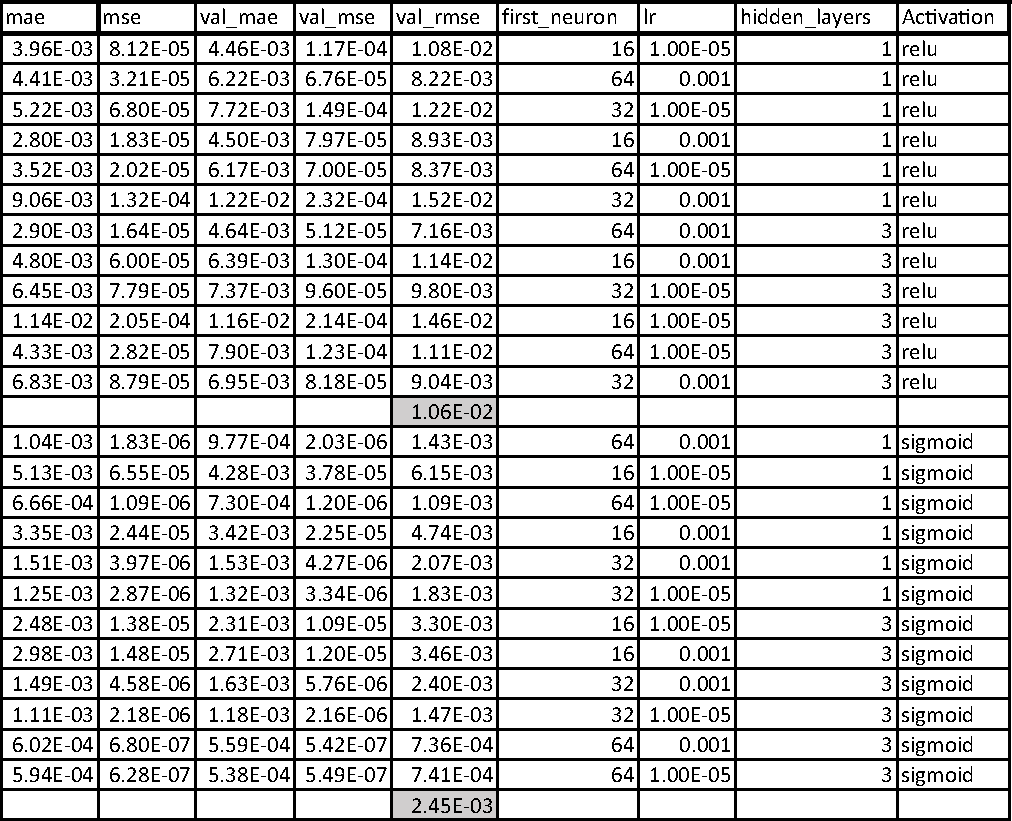
\includegraphics[width=9cm]{gridsearch.pdf}
	\caption{Grid search. Manipulated Hyperparameters include activation function, number of layers, density of layers, learning rate. Activation function had the largest effect as expected}
	\label{fig:gridsearch}
\end{figure}

Fig. \ref{fig:ilrresults} shows the results of function approximating with ILR. It is clear that when the sample-to-feature ratio approaches two, the error exponentially ramps upwards. It can also be observed that for sample-to-feature ratios above five, the results are very similar. This suggests that there is a statistically significant sample-to-feature roof for ILR around five, which permits an empirical selection of samples when given the number of features by the user.

\begin{figure}[h]
	\centering
	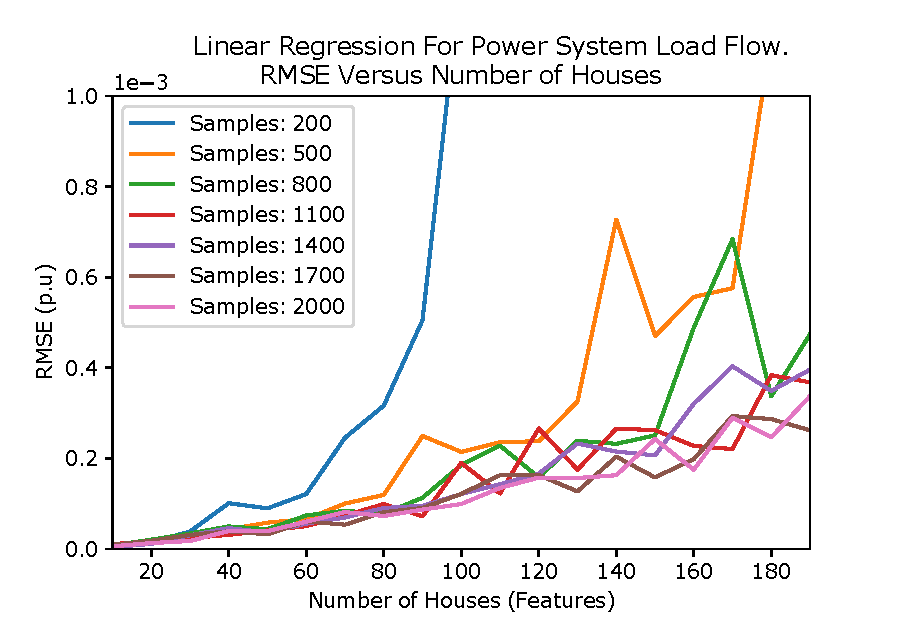
\includegraphics[width=9cm]{ilrrmsevsfeatures_familyofcurves.pdf}
	\caption{ILR for PSLF equations with various input features spaces and sample}
	\label{fig:ilrresults}
\end{figure}

The results in Fig. \ref{fig:annresults} show that the nonlinear ANN solution produces more error than the ILR fit. This would suggest that the PSLF has extremely little noise, even when the feature space is as large as 200 dimensions. Further hyperparameter tuning should result in better ANN results but may require a potentially unrealistic amount of time. One interesting observation from the figure is the approximation results are much more sporadic when the samples-to-feature ratio is below five. It confirms that the nonlinear solution requires more data than the ILR to be trained to a low RMSE, which is to be expected \cite{gema1992}.

\begin{figure}[h]
	\centering
	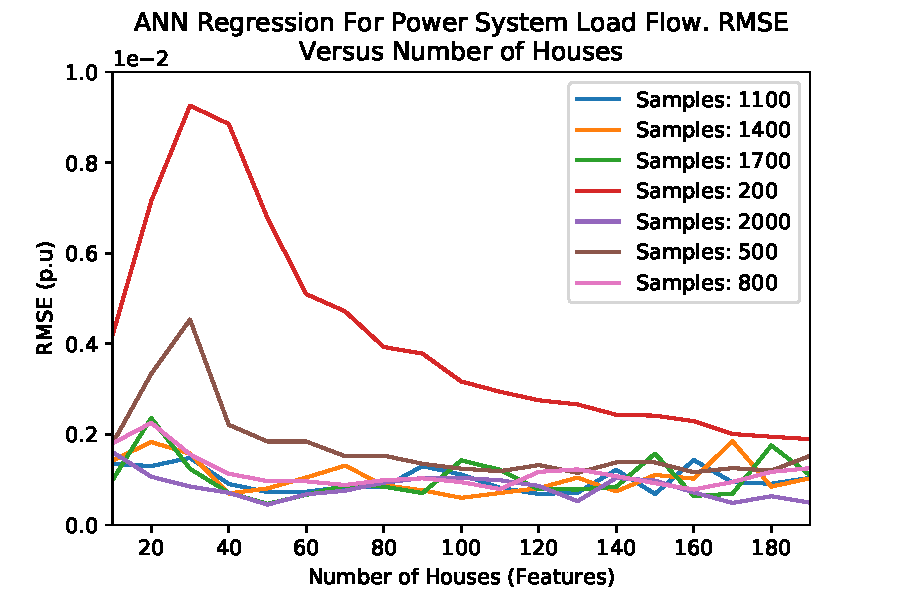
\includegraphics[width=9cm]{annrmsevsfeatures_familyofcurves.pdf}
	\caption{ANN for PSLF equations with various input features spaces and samples}
	\label{fig:annresults}
\end{figure}

Fig. \ref{fig:comparison} visualises the accuracy of function approximating with both ILR and ANN mappings for one node in a 500 house radial power system network	. The ILR and ANN RMSE were 0.0021 and 0.0019 respectively.

\begin{figure}[h]
	\centering
	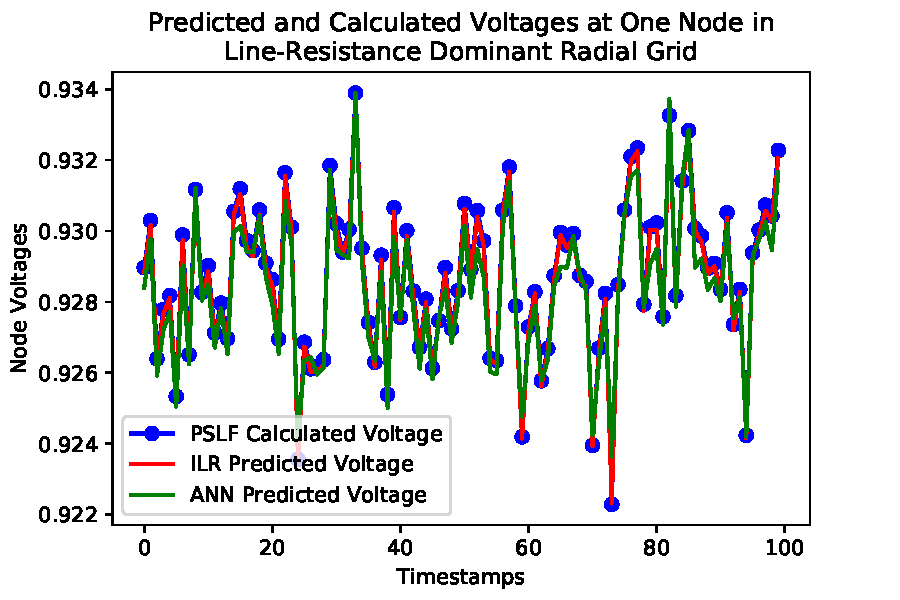
\includegraphics[width=9cm]{comparingvoltages_500.pdf}
	\caption{Comparison of voltage profiles: PSLF calculated, ILR approximated and ANN approximated. Radial network included 500 houses}
	\label{fig:comparison}
\end{figure}

\section{Conclusions}
\label{sec:conc}
In this paper, multiple function approximation techniques are applied to a PSLF equation. The ILR outperformed the ANN-based nonlinear regression which was contrary to the original hypothesis. More hyperparameter tuning would likely deliver better ANN results, but it is unclear how long it would take to decrease RMSE by at least two orders of magnitude, which would make it outperform the ILR solution according to the results in Fig. \ref{fig:ilrresults} and Fig. \ref{fig:annresults}. A hyperparameter search suggests using sigmoid activation functions and increasing layer density would be the best approach. Consideration of the extrema in the feature space moment could lead to an analytical selection of ANN hyperparameters. Further studies should include other features common to power system topologies found in Table. \ref{table:sim model}.

\section*{Acknowledgment}
Support from Future Energy Systems under the Canada First Research Excellence Fund (CFREF) at the University of Alberta is humbly appreciated.


\bibliography{2019_ccece}
\bibliographystyle{IEEEtranN}

\end{document}

